\chapter{Conclusion and Future Work}
\label{sec:conclusion_future_work}

- Die numerischen Fehler während der Simulation des Heston-Models mittels QE-Schema konnten identifiziert und ausgeschlossen werden. Es stellte sich heraus, dass, wenn die Feller condition zu stark nicht erfüllt war, diese Fehler auftauchten. Andersen (2008) schreibt aber in seinem Paper, dass das QE-Schema auch in solchen Fällen funktioniert, es kann sich also nur um einen Fehler in der Implementierung handeln. Tatsächlich konnte dieser Fehler zum Ende dieser Arbeit gefunden und behoben werden, die Zeit reichte aber nicht mehr aus, um diese Simulationen neu durchrechnen zu lassen. Problem war die Berechnung der Gleichung \eqref{eq:qe_dirac} und das Ziehen von $U_v$ aus der uniform distribution. Falls $U_v$ dort exakt den Wert 1 annimmt, so wird zur Berechnung von $\Psi^{-1}$ durch 0 geteilt, was zu dem Fehler führt. Das kommt aber nur zum Tragen, wenn $v_t$ sehr klein ist und bleibt, also die Feller condition stark nicht erfüllt ist. Das Ziehen von $U_v$ wurde so angepasst, dass es zwischen $10^{-10}$ und $1-10^{-10}$ liegt. Einige kurze Tests haben gezeigt, dass dieser Fehler damit behoben ist.

- Trotz der beschränkten Aussagekraft von Simulationen mit $\mu=0.05$ habe ich einen 3D-Plot erstellt, der darstellt, wie gut die Gram-Charlier-Expansion auf der Basis von Cumulanten die theoretische Verteilung gut (p value $>5\%$) approximiert.
- Wir können schauen, wie sich der Pairplot Abbildung \ref{fig:pairplot_GC_cum_KS_muzero} ändert, wenn wir $\mu=0.05$ setzen (see Abbildung \ref{fig:pairplot_GC_cum_KS_mu005}). Es fällt direkt auf, dass es weiße Stellen im Diagramm gibt. Das sind die Fälle, bei denen durch das Herausfiltern aller ungültigen Simulationen keine Simulationen mehr übrig bleiben. Das ist immer dann der Fall, wenn die Feller condition stark nicht erfüllt ist, also $2\kappa\theta - \sigma^2 <0$. Interessant ist, dass dieser Effekt nur bei $\mu=0.05$ so stark zum Tragen kommt, bei $mu=0$ fielen nicht so viele Simulationen weg.
- Der andere, sehr überraschende Punkt ist, dass es insgesamt mehr gelbe Punkte gibt, die Gram-Charlier-Expansion sich also -- für passend gewählte Parameter -- besser an die theoretische Verteilung annähert, wenn der Preisprozess kein Martingale ist. Im Gegenzug gibt es aber auch mehr Parameterkombinationen (insbesondere $\sigma$, $\kappa$ und $\theta$), bei denen sich die Gram-Charlier-Expansion schlechter an die theoretische Verteilung annähert.

\begin{figure}
    \centering
    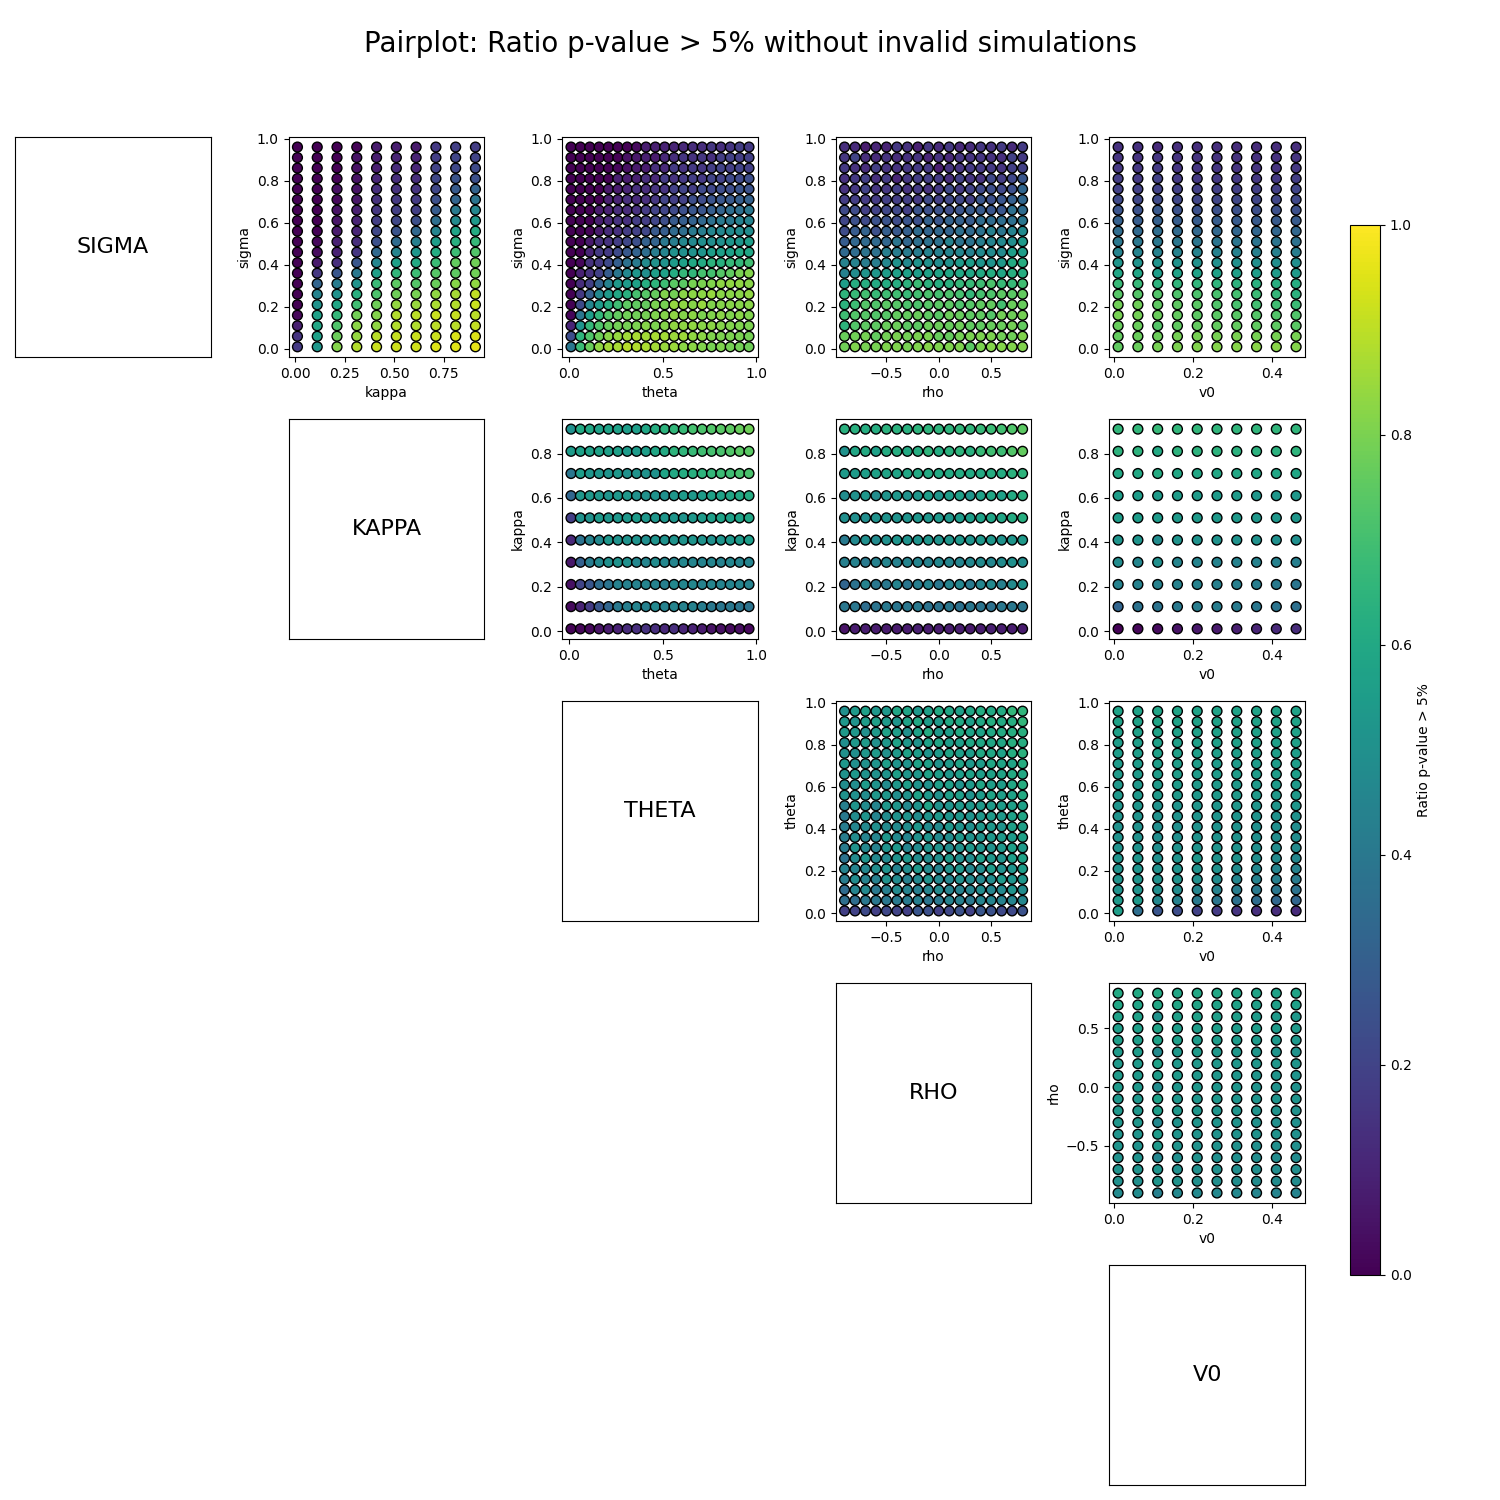
\includegraphics[width=0.8\textwidth]{img/pairplot_GC_cum_KS.png}
    \caption{Pairplot for each pair of parameters for the Heston Model and the percentage of p values of the Kolmogorov-Smirnov-Test for the Gram-Charlier Expansion with Cumulants vs the theoretical density above 5\%. Invalid simulations are excluded and $\mu=0.05$.}
    \label{fig:pairplot_GC_cum_KS_mu005}
\end{figure}

\begin{figure}
    \centering
    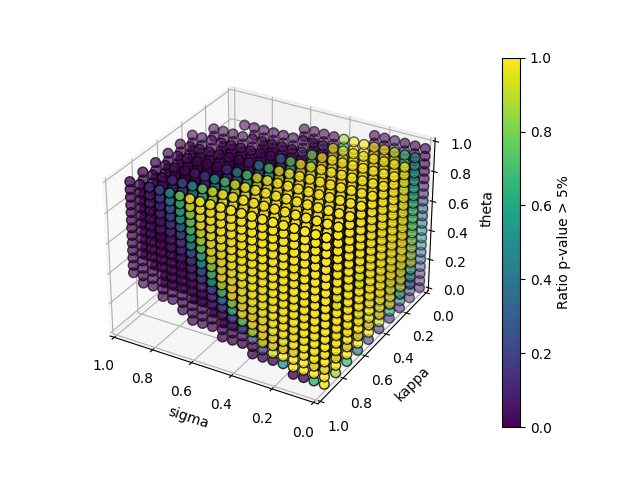
\includegraphics[width=0.8\textwidth]{img/GC_cum_KS_3d_p_value_sigma_kappa_theta.png}
    \caption{Percentage of simulations where the p-value of the Kolmogorov-Smirnov-Test against the theoretical density is above 5\%. Invalid simulations are excluded. $\mu=0.05$}
    \label{fig:GC_cum_KS_3d_p_value_sigma_kappa_theta_mu005}
\end{figure}

- In der detaillierteren Darstellung \ref{fig:GC_cum_KS_3d_p_value_sigma_kappa_theta_mu005} sieht man besonders deutlich den Unterschied zwischen $mu=0$ (Abbildung \ref{fig:GC_cum_KS_3d_p_value_sigma_kappa_theta_muzero}) und $mu=0.05$ (Abbildung \ref{fig:GC_cum_KS_3d_p_value_sigma_kappa_theta_mu005}). Es ist bisher unklar, warum die Gram-Charlier-Expansion bei $\mu=0.05$ zu teilweise besseren Ergebnissen kommt und ob sich dieser Effekt auch bei anderen Werten von $\mu$ zeigt. Hier könnte zukünftige Forschung ansetzen.